\chapter{Modelling an Insurance Group}\label{chap:insuranceGroup}

As is the case for single corporations, the consolidated insurance group must meet group
solvency regulatory requirements to preserve financial stability of the group and protect
policy holders and beneficiaries.\footnote{An \term{Insurance Group} consists of several
insurance companies, while an \term{Insurance Conglomerate} must own both insurance and
banking companies.}
Within the European Union, large-scale changes are in progress based on the proposal of the
Solvency~II Framework Directive, entailing a shift of competence for group supervision from
national solo-supervisory authorities to a genuine Group Supervisor on the European level
~(\cite{07:CEANoteSolv2Groups,08:FinMaCircular29,08:Sehrbrock,06:FSAdiscussionPaper}).

There are currently two internationally prevalent approaches to modelling relevant group
risks, exhibiting varying perspectives. A very nice outline of the basic principles of these
approaches is given in Circular~2008/44 of FinMa (\cite{08:FinMaCircular44,08:FinMaCircular44_de}), 
from which we quote:

\begin{quote}

The first approach models the risks of a group on a consolidated basis as if the group were
a single legal entity (``consolidated group modeling"). As a consequence, the lead
supervisor can determine whether the group satisfies capital adequacy requirements as based
on its external liabilities. In so doing, intra-group liabilities are not modeled as it is
implicitly assumed that assets are freely transferable within the group.

The second approach is based on modeling the risks of the individual legal entities of a
group, possibly forming a cluster, and thus models the relations between these units in
addition to the external relations (``granular group modeling"). In this second method
uniform rules are applied to assess the risks of the assets and liabilities of the
individual legal entities, in addition to the risks resulting from the relations within the
group. This second method enables \FinMa, in its capacity of lead supervisor of the group,
to determine whether any risk potential is posed to policyholders and the financial
stability of the group by individual parts of the group itself for other parts of the group
or for the group as a whole, and whether the individual parts of the group aid the others as
needed or whether other risk-mitigating measures are available.

In the \SST{} it is assumed that granular group modeling is applied, with consolidated group
modeling additionally being permitted upon application by the group with \FINMA{} or being
requested by \FINMA{}. The ``group SST" is based on granular group modeling, which can be
supplemented by consolidated group modeling.
\end{quote}

The ``Multi Company Model" provided by \RA{} may serve as an appropriate internal model for
granular determination, quantification, and analysis of all relevant risks of insurance
conglomerates.  In what follows we discuss the implementation of the model, its findings in
extension to the \PODRA{} model, and the internal processing of data related to specific group
segments.  Instructions for creating a parametrization in the group model are given in
Chapter~\ref{chap:multiCompany}.

%The first approach pictures the risks of a group on a consolidated basis, that is, losses
%and franking balances remain with the consolidated group on an entity's (``consolidated
%group modeling"). Therewith only external liabilities are modeled rather than group
%internal liabilities, as it is implicitly supposed that asset values within the group may
%be transferred freely.

%The second approach is based on risk modeling of the individual legal units of a group of
%corporations, if need be subsumed to a cluster, and pictures additionally to the external
%relations the relations between these units (``granular group modeling"). Granular group
%modeling not only allows to estimate the risks of assets and liabilities of the individual
%corporate bodies, but also to capture the risks resulting from the relations within the
%group entity called {\em intra-group relations} in the following.


%losses and franking balances
%remain with the consolidated group on an entity's

\section{Company Segments}\label{sec:companySegments}
As usual, a new insurance company may be created by right-clicking on \term{Companies} and
selecting \term{Add} in the appearing context menu.
Another possibility is to right-click on an existing company and choose \term{Duplicate} in
the context menu leading to a one-to-one copy of the existing segment. Each company segment
consists of a rating parameter that has to be selected from a list with rating values
ranging from \term{AAA} to \term{D}. Rating parameters play an important role for the
quantification of contingency risks, particularly in regard to the Solvency~II Framework
a precautionary approach in selecting business partners should be taken. To this end,
credit-worthiness and solvency information from rating agencies may serve as an important
mean to guarantee long-term competitive advantages. For a comprehensive discussion about
the importance of rating for reinsurances, the interested reader is referred
to~\cite{09:MunichReRating}.

Each predefined company segment represents a legal entity\footnote{Or a so called
\term{Cluster}, \ie~well-defined set of legal entities. Clustering is usually allowed for
non-significant legal entities or where some legal entities cover the same risk but consist
of two carriers. The latter might be the case if one legal entity is funded by a SPV ("Special Purpose Vehicle"); or for
fully fronted business.} belonging to the insurance group built by the union of all the
company segments.
Hence, in contrast to the \PODRA{} model that provides a tool for modeling the exposure of one
insurance company only, we now have to specify the respective insurance unit when editing
risks, reinsurance contracts, etc.
In so doing, we obtain a consistent possibility of correct valuation of the assets and all
liabilities of all the legal units of the insurance group and modeling all the relevant
risks of the individual legal units.
In view of the fact that capital and risk transfers, such as loans or reinsurance contracts,
are frequently used among the legal entities of an insurance group, the ``Multi Company
Model" provides an important and sound base for managing the risks of groups on a granular
perspective level.

The feature of including multiple legal units into the model exhibits its utility after
running the simulation and opening the preselected result descriptor. For the sake of
illustration we will consider an example below, for starters we focus on the result 
template as shown in Figure~\ref{fig:multiCompany-results}.

\begin{figure}[htb]
	\centering
	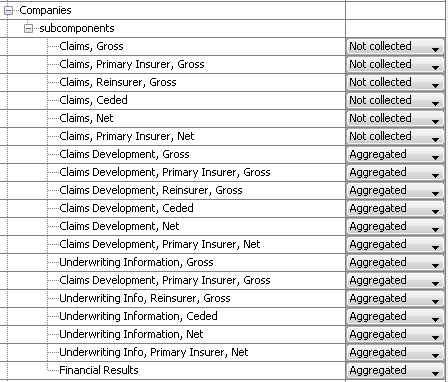
\includegraphics[scale=0.7]{images/multiCompany_companiesResult.png}
	\caption{\term{MultiCompany}: Results for segments of component \term{Companies}}
	\label{fig:multiCompany-results}
\end{figure}

In the template we nicely see that the result descriptor shows the activities of each of the
single units of the group separately. As outlined in
Chapter~\ref{chap:riskAnalyticsApplication} the model does not define which output variables
have to be collected during the simulation.
Instead, the user has to determine before starting the simulation if at all and to which
granular level (ranging from the coarse-grained \term{Aggregated} to the fine grained
\term{Single}) he wants to collect each of the positions listed below
\term{subcomponents} (which is a placeholder for the single entities).
The items that are shown in the result tree-view may be roughly separated into claims,
underwriting information and financial results.
In order to apply the model correctly we have to understand how the resulting items listed
in Figure~\ref{fig:multiCompany-results} are fed into the company segments. This is
explained in full detail in Section~\ref{sec:processing}.
Another issue worth discussing is how claims\footnote{We restrict to claims and
note that the following discussion applies to the developed claims as well.} and
underwriting information are split up into
\begin{itemize}
	\item gross claims and gross underwriting information,
	\item gross claims of primary insurer and gross underwriting information of primary insurer,
	\item gross claims of reinsurer and gross underwriting information of reinsurer,
	\item ceded claims and ceded underwriting information,
	\item net claims and net underwriting information, and
	\item net claims of primary insurer and net claims of reinsurer.
\end{itemize}
This breakup of information is rooted in the fact that an insurance company 
\footnote{We speak here of a single unit of the group and NOT of the group as an entity.} %
may be fully licensed to transact general primary insurance {\em and} reinsurance business.

We close this section by exemplifying the aforementioned matter by means of three imaginary
companies \dquot{Mars Re}, \dquot{Venus} and \dquot{Pluto Re}, each of them trading in the
primary- as well as re-insurance business.
At first view the set up of the example may be a disincentive to the user, however in
anticipation of the following section it also gives an idea of the internal handling of
information. As will be clear below, the example is constructed as a small tutorial where the user 
is requested to create a parametrization in \PillarOne{} leading to a simulation model that renders the 
outlined results. 

\example{
The three insurance companies \dquot{Mars Re}, \dquot{Venus} and \dquot{Pluto Re} are
trading in different classes of business, contingently purchasing reinsurance from one or
several reinsurers. The contracts (direct business with related reinsurance contracts) are
shown in Table~\ref{table:exampleCompanies} below, where each column belongs to one class of
business.

\begin{table}[htb!]\small
\centering
\resizebox {0.9\textwidth }{!}{
\begin{tabular}{|l||l||l||l||l|}
\hline
\rule{0pt}{4ex} {\textbf{line of business:}} & {motor Venus} & {motor Mars Re} & {motor Pluto Re} & {accident Mars Re} \\
\hline
\rule{0pt}{4ex} {\textbf{direct insurer:}} & {Venus} & {Mars Re} & {Pluto Re} & {Mars Re}\\
\hline
\rule{0pt}{4ex} {\textbf{reinsurance treaty:} }&{ QS motor Venus} & {QS motor Mars} & {---}& {QS accident Mars}\\
\hline
\rule{0pt}{4ex} {\textbf{reinsurer:}} & {Mars Re} & {---} & {---} & {Pluto Re: 0.7,\,Venus: 0.3}\\
\hline
\end{tabular}}
\caption{Insurance business activities and contractual relationships}
\label{table:exampleCompanies}
\end{table}

Note that the last entry in the last column denotes a reinsurance contract that is shared
between two reinsurers registered with associated portions.
Moreover the line of business ``motor Pluto Re" has no specified reinsurance contracts,
whereas ``motor Mars Re" reinsures its business but with an reinsurer that is unknown
here\footnote{This corresponds exactly to the parametrization where the user is not forced
to select a reinsurer from the list of companies in contrast to the lines of business
component.}.
Having listed all the necessary information, we may process the incoming information of
claim burdens and underwriting segments and allocate it to the predefined companies.
In the next two tables we give a list of all the incoming gross and ceded information
allowing for calculating the profit of each of the three companies in the group.

\begin{table}[htb!]
\centering
\scalebox {0.6}[0.6]{
\begin{tabular}{|l|l|l|}
\hline
\rule{0pt}{4ex} & \textbf{written premium} & \textbf{line of business} \\
\hline
\rule{0pt}{4ex} {\textbf{packet 1}} & 1 mio & {motor Venus} \\
\hline
\rule{0pt}{4ex} {\textbf{packet 2}} & 2 mio & {motor Mars Re}\\
\hline
\rule{0pt}{4ex} {\textbf{packet 3} }&0.5 mio & {motor Venus}\\
\hline
\rule{0pt}{4ex} {\textbf{packet 4}} &1.8 mio & {accident Mars Re} \\
\hline
\rule{0pt}{4ex} {\textbf{packet 5}} &0.05 mio &{motor Pluto Re} \\
\hline
\end{tabular}\hspace{0.6cm}
\begin{tabular}{|l|l|l|l|l|}
\hline
\rule{0pt}{4ex} & \textbf{ceded written premium} & \textbf{line of business} &\textbf{reinsurance contract}&\textbf{commission}\\
\hline
\rule{0pt}{4ex} {\textbf{packet 1}} & 0.1 mio & {motor Venus} & QS motor Venus & -0.02 mio \\
\hline
\rule{0pt}{4ex} {\textbf{packet 2}} & 0.4 mio & {motor Mars Re}& QS motor Mars& -0.04 mio\\
\hline
\rule{0pt}{4ex} {\textbf{packet 3} }&0.05 mio & {motor Venus}& QS motor Venus &-0.01 mio\\
\hline
\rule{0pt}{4ex} {\textbf{packet 4}} &0.9 mio & {accident Mars Re} & QS accident Mars&-0.45 mio\\
\hline
\end{tabular}}
\caption{\footnotesize{\textbf{Incoming underwriting information:} gross info (left side), ceded info (right side)}}
\label{table:underwritingInfo}
\end{table}

\begin{table}[htb!]

\centering
\scalebox {0.6}[0.6]{
\begin{tabular}{|l|l|l|}
\hline
\rule{0pt}{4ex} & \textbf{claims} & \textbf{line of business} \\
\hline
\rule{0pt}{4ex} {\textbf{packet 1}} & 1.5 mio & {motor Venus} \\
\hline
\rule{0pt}{4ex} {\textbf{packet 2}} & 1.0 mio & {motor Mars Re}\\
\hline
\rule{0pt}{4ex} {\textbf{packet 3} }&0.2 mio & {motor Venus}\\
\hline
\rule{0pt}{4ex} {\textbf{packet 4}} &1.2 mio & {accident Mars Re} \\
\hline
\rule{0pt}{4ex} {\textbf{packet 5}} &0.04 mio &{motor Pluto Re} \\
\hline
\end{tabular}\hspace{0.6cm}
\begin{tabular}{|l|l|l|l|}
\hline
\rule{0pt}{4ex} &\textbf{ceded claims} &\textbf{line of business} &\textbf{reinsurance contract}\\
\hline
\rule{0pt}{4ex} {\textbf{packet 1}} & 0.15 mio & {motor Venus} & QS motor Venus \\
\hline
\rule{0pt}{4ex} {\textbf{packet 2}} & 0.2 mio & {motor Mars Re}& QS motor Mars\\
\hline
\rule{0pt}{4ex} {\textbf{packet 3} }& 0.02 mio & {motor Venus}& QS motor Venus \\
\hline
\rule{0pt}{4ex} {\textbf{packet 4}} &0.6 mio & {accident Mars Re} & QS accident Mars\\
\hline
\end{tabular}}
\caption{\footnotesize{\textbf{Incoming claims burden:} gross claims (left side) and ceded claims(right side)}}
\label{table:claims}
\end{table}

The attentive reader may have noticed that underwriting information for the line ``motor
Venus" is listed twice in Table~\ref{table:underwritingInfo}. This may result, \eg from a
partition into motor third party and motor comprehensive cover\footnote{We are aware of the
fact that subsuming such segments under one line of business is a rather `quick and dirty'
approach.}.
As an exercise we evaluate the results for the single insurance units of the group that will
be shown in the result descriptor when the collector \term{Aggregated} is selected.
To this end, the reader is invited to 
\begin{enumerate}
\item compute the results by hand in order to understand the
specific characteristic of \term{Companies} and, 
\item to practice the handling of the simulation tool by filling the parametrization form of the ``Multi Company
Model" with parameters and values reflecting the situation given in
Tables~\ref{table:exampleCompanies},~\ref{table:underwritingInfo} and~\ref{table:claims}.
\end{enumerate}
After running the simulation the results can be taken from the result template.
In Figure~\ref{fig:resultsMarsPluto} the aggregated results are illustrated for the
insurances ``Mars Re" and ``Pluto Re", while for ``Venus" the problem is accomplished
step-by-step.

\begin{figure}[htb]
\centering
\subfloat[Aggregated results for ``Mars Re"]{
\label{fig:subfig:mars}
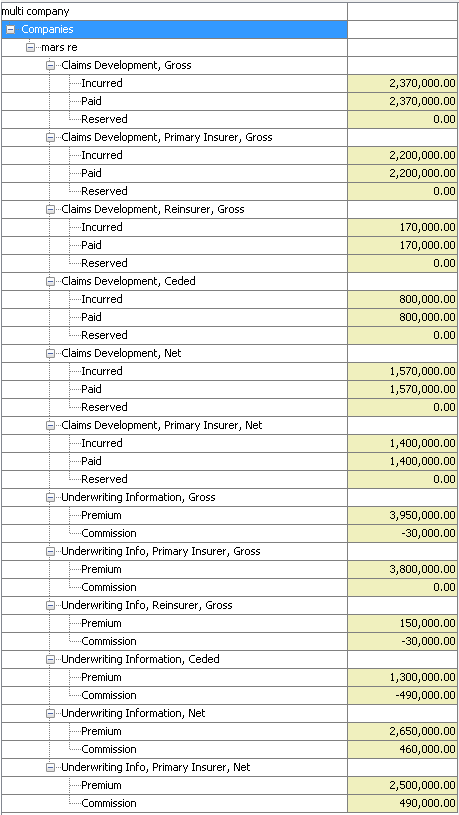
\includegraphics[scale=0.6]{images/exampleMarsRe.png}}
\hspace{1cm}
\subfloat[Aggregated results for ``Pluto Re"]{
\label{fig:subfig:pluto}
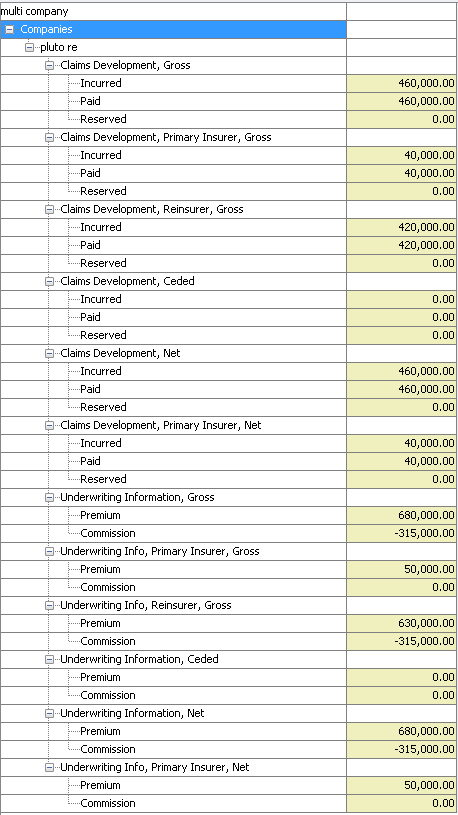
\includegraphics[scale=0.6]{images/examplePlutoRe.png}}
\caption{Simulation results corresponding to example}
\label{fig:resultsMarsPluto}
\end{figure}


We start our considerations with the remark that the business activity of an insurance
company is quantified by merging operations in the direct insurance business with the
reinsurance business implying for the example that ``Venus" not only obtains premiums from
the left-sided list in Table~\ref{table:underwritingInfo}, but also from possible
reinsurance business listed on the right-hand side of Table~\ref{table:underwritingInfo}.
Explicitly: Subsequently using the monetary unit one million, the total gross premium
$P_{\mathrm{gross}}$ of ``Venus" is derived as the sum\footnote{We use the abbreviations PI
and RI for primary insurer and reinsurer, respectively.}
\begin{equation*}
P_{\mathrm{gross}}= P_{\mathrm{gross}}^{\scriptscriptstyle{(PI)}}+
P_{\mathrm{gross}}^{\scriptscriptstyle{(RI)}}\,,
\qquad\quad P_{\mathrm{gross}}^{\scriptscriptstyle{(PI)}}\,=
\,1.5\,,\qquad P_{\mathrm{gross}}^{\scriptscriptstyle{(RI)}}\,=
\,0.27\,,
\end{equation*}
where $P_{\mathrm{gross}}^{\scriptscriptstyle{(RI)}}$ originates from the cession of the
business line ``accident Mars Re" ($0.9$ ceded premium) weighted with the ``Venus"-share of
$0.3$ in the reinsurance treaty.
The resulting net premium $P_{\mathrm{net}}=P_{\mathrm{gross}}-P_{\mathrm{ceded}}$ then
results by subtracting from $P_{\mathrm{gross}}$ the total of ceded premiums
$P_{\mathrm{ceded}}=0.15$ of ``Venus", and reporting also the direct insurer's portion
$P_{\mathrm{net}}^{\scriptscriptstyle{(PI)}}$ of the net premium, we end up with
\[  P_{\mathrm{net}} \,=\,1.62 \,,\qquad\qquad  P_{\mathrm{net}}^{\scriptscriptstyle{(PI)}}\,=\,1.35\,.\]
Note that the net results are not reported for exclusive reinsurance business as by
definition and excluding retrocession\footnote{At this stage \PillarOne{} does 
not allow for cover strategies that apply to predefined reinsurance contracts.}
 it corresponds to
$P_{\mathrm{gross}}^{\scriptscriptstyle{(RI)}}$.

In the same way we handle the designated commission where it is clear that the commission in gross portfolios of direct insurance
business is zero by default. Moreover notice about the sign convention for commissions that becomes 
clear when compared to premiums. Following the guidance for premiums we then obtain for gross, ceded and net commissions
$C_{\mathrm{gross}},\,C_{\mathrm{ceded}},\,C_{\mathrm{net}}$
\[  C_{\mathrm{gross}}\,=
\,-0.135\,,\quad C_{\mathrm{ceded}}\,=\,-0.03 \,,\quad
C_{\mathrm{net}}\,=\,C_{\mathrm{gross}}-C_{\mathrm{ceded}}\,=\,-0.105\,.\]
Splitting these results into exclusive reinsurance and primary insurance business yields
\[ C_{\mathrm{gross}}^{\scriptscriptstyle{(RI)}}\,=
\,C_{\mathrm{gross}}\,,\qquad\quad
C_{\mathrm{net}}^{\scriptscriptstyle{(PI)}}\,=-C_{\mathrm{ceded}}\,. \]
Table~\ref{table:claims} finally supplies the results for the claims (or losses) denoted by
$L$. Using the above rules for sub- and super-indexing we end up with
\begin{eqnarray*}
L_{\mathrm{gross}} & = & L_{\mathrm{gross}}^{\scriptscriptstyle{(PI)}} +
L_{\mathrm{gross}}^{\scriptscriptstyle{(RI)}}\,,\qquad L_{\mathrm{gross}}^{\scriptscriptstyle{(PI)}}\,=
\,1.7\,,\qquad L_{\mathrm{gross}}^{\scriptscriptstyle{(RI)}}\,=
\,0.18
\end{eqnarray*}
for the gross losses, $L_{\mathrm{ceded}}=0.17$ for ceded claims and
\begin{eqnarray*}
L_{\mathrm{net}} & = &  L_{\mathrm{gross}} -L_{\mathrm{ceded}}\,=\, 1.71\,,\qquad
L_{\mathrm{net}}^{\scriptscriptstyle{(PI)}}\,=\, L_{\mathrm{gross}}^{\scriptscriptstyle{(PI)}}-L_{\mathrm{ceded}}\,=\, 1.53\,.
\end{eqnarray*}
for net results.
}
% Here ends the example

\section{Internal Processing of Data}\label{sec:processing}

\todo{}{Where to place this section?}
For the understanding of the model it is of utmost importance to get an overall picture of
the internal handling of the information stemming from the parametrization defined by the
user.  We will now discuss this issue in full detail with the help of the \term{Companies}
component processing information about claims, underwriting segments, and financial results.

The value of \term{Financial Results} as listed in Figure~\ref{fig:multiCompany-results}) is
evaluated in a direct way using the fact that each segment of \term{ALM Generators} has a
parameter \term{Company} forcing the user to attach to one segment of \term{Companies}.
By this means progression is straightforward in that each segment of \term{ALM Generators}
generates output value(s) stored in a variable that is marked with the associated company.
We finally obtain a list of results collecting outputs of all the ALM segments.
In a next step this list is sent to all segments of the component \term{Companies}.
To put it roughly, for each of these segments the incoming list is filtered with respect to
the company-marker that is attached to the result variables.
If the company under consideration is \dquot{Venus} we will pass through the list and
collect all results that are marked with company \dquot{Venus}, whereas the leftover is
discarded.  The \dquot{Venus}-labeled results are summed up and finally prepared by the
dedicated result descriptor.

Handling of gross claims is slightly more sophisticated in that segments of \term{Claims
Generators} are not attached to the component \term{Companies} directly.
Instead, interrelation is given indirectly via the component \term{Lines Of Business} acting
as a kind of intermediary.
As nicely illustrated in Figure~\ref{fig:multiCompany}, each segment of \term{Lines of
Business} has two parameters that are of interest here:
The parameter \term{Company} attaching the participating insurance unit to the dedicated
business line, and the parameter \term{Line of Business Claims} -- \term{\em Shares}
providing the link between segments of \term{Companies} and \term{Claims Generators}.
Figures~\ref{fig:processingGrossClaims} and \ref{fig:processingCededClaims}
\todo{}{This and the next figure need a revision. I am open for suggestions!}
give a rough sketch of internal handling of the data that is based on the component-coupling
as outlined before.
\begin{figure}[htb]
	\centering
	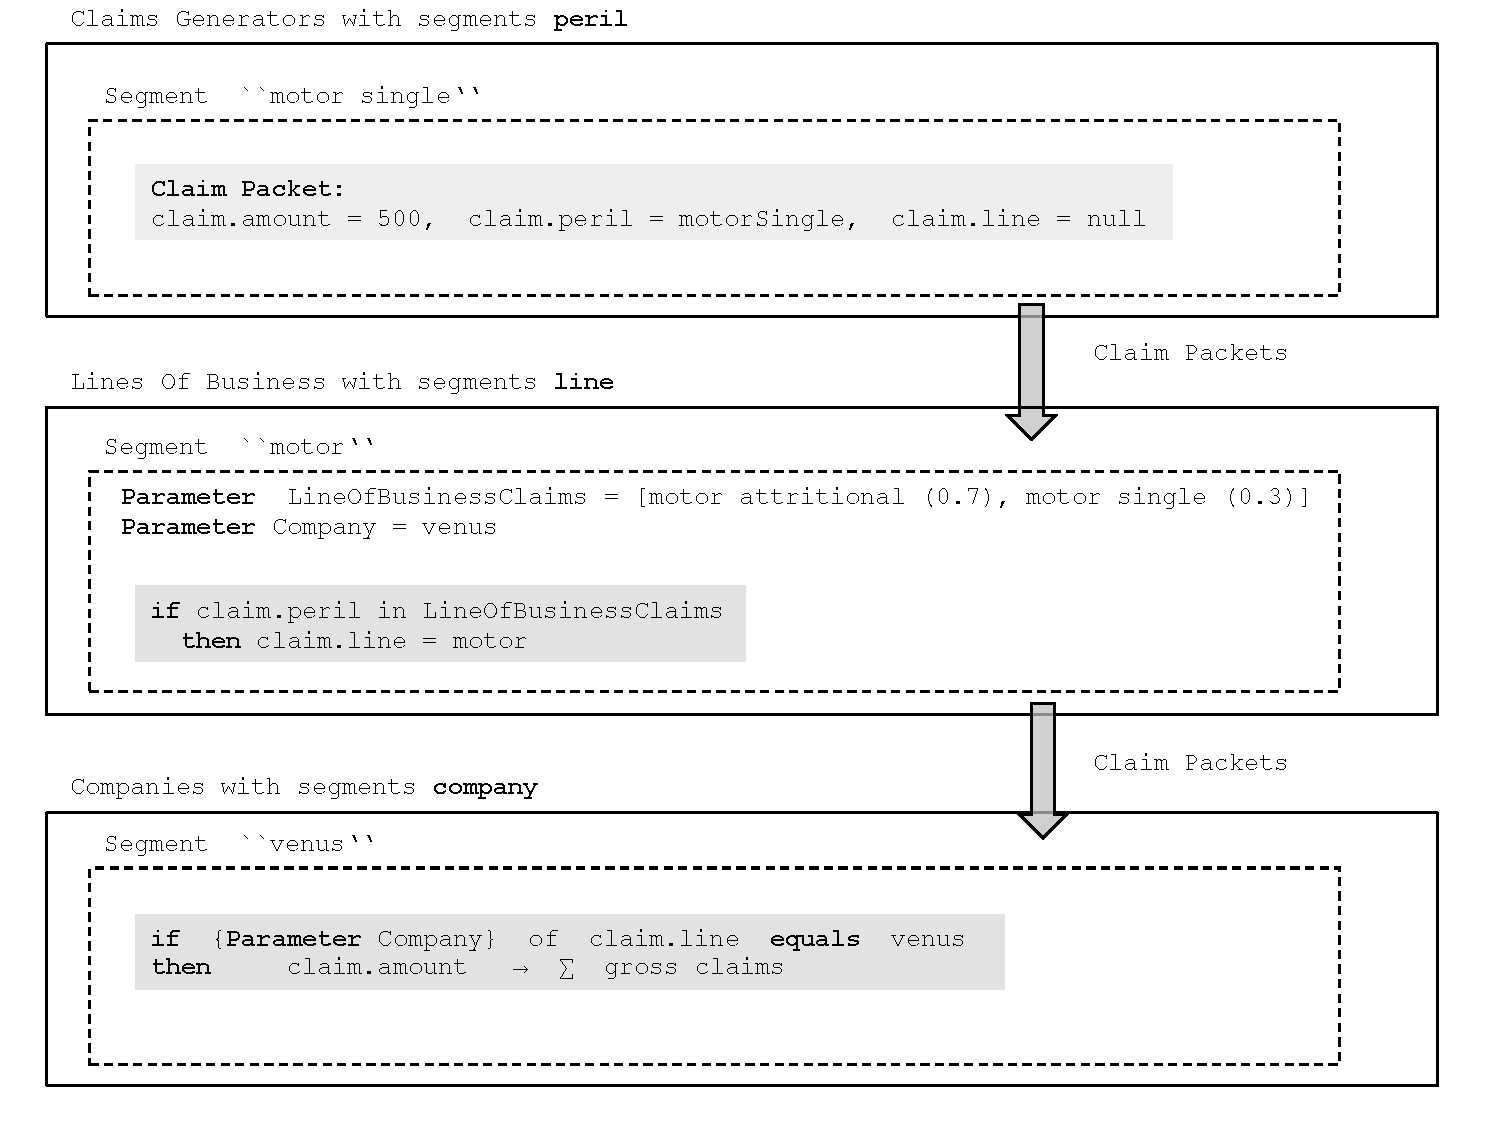
\includegraphics[scale=0.45]{images/ProcessingGrossClaims.pdf}
	\caption{Internal handling of gross claims in \term{Companies}}
	\label{fig:processingGrossClaims}
\end{figure}
With these preparations it is easy to understand how gross claims are processed:
The claim packets are sent to all of the objects of \term{Lines of Business}, where their
member variable {\em claim.line} is instantiated with the business line under consideration
if and only if it is related to the peril (that is, the origin of the claim) by means of the
parameter \term{Line of Business Claims}. Hence filtering of claims in the company segments
is carried out by means of the member variable {\em claim.line} pointing to the business
line with assigned parameter \term{Company}.
For managing of ceded claims we refer to Figure~\ref{fig:processingCededClaims} and remark
that underwriting information is processed analogously to claims by using the component
\term{Underwriting} rather than
\term{Claims Generators} (compare Figure~\ref{fig:multiCompany}).
\begin{figure}[htb]
	\centering
	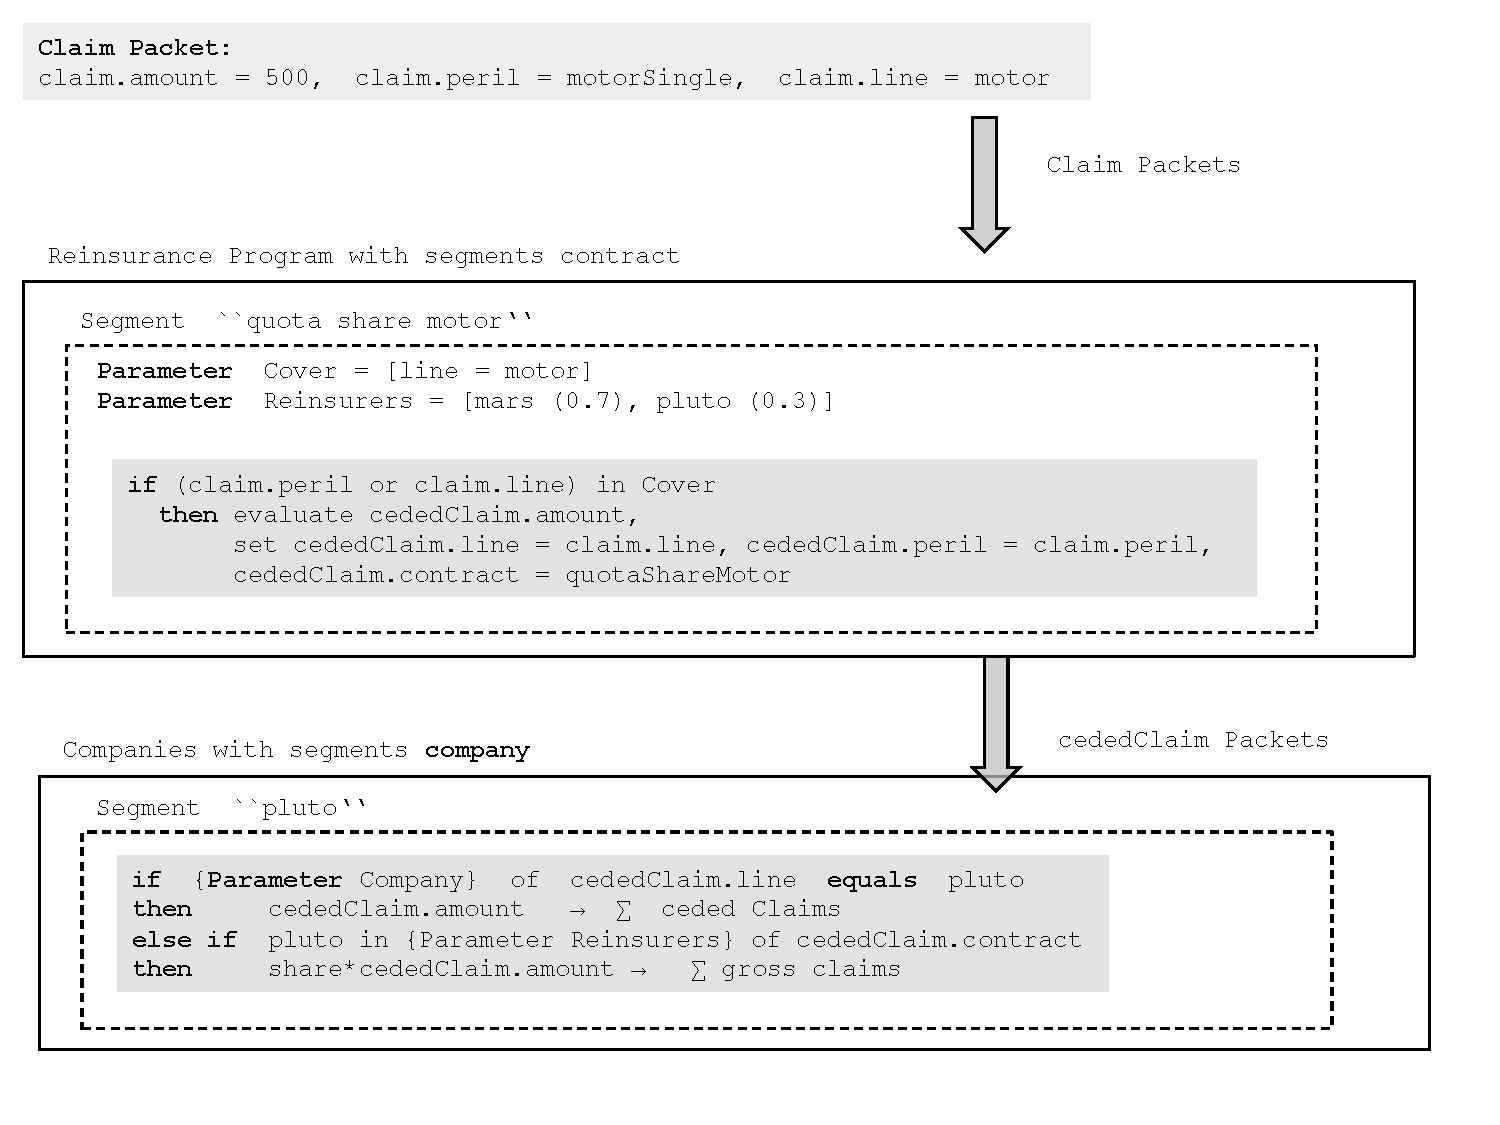
\includegraphics[scale=0.45]{images/ProcessingCededClaims.pdf}
	\caption{Internal handling of ceded claims in \term{Companies}}
	\label{fig:processingCededClaims}
\end{figure}
